\chapter{Úvod}
\blind{3}

\chapter{Teorie}


\section{Jazykové modely}

\todo{jazykove modely v kontextu machine translation, generovani jazyku}

\subsection{N-gram}
\subsection{log-linear}

\section{Neuronové sítě?}

\section{Rekurentní neuronové sítě}
V této kapitole je popsán základní koncept rekurentních neuronových sítí (RNN\footnote{z anglického recurrent neural network}), jejich srovnání s běžnými neuronovými sítěmi a dále pak popis upravených variant RNN -- LSTM \ref{section:LSTM} a GRU \ref{section:GRU}. Kapitola volně vychází z práce \cite{nmtThesis}.\\


RNN (Elman \cite{rnn}) jsou známé již přes dvě desítky let. Úspěšně jsou však používány až v posledních letech a to hlavně díky vyššímu výpočetnímu výkonu a většímu objemu trénovacích dat, který je v současné době dostupný a také, díky většímu výkonu, zpracovatelný. Tento druh neuronových sítí je obzvlášť vhodný například pro rozpoznávání psaného písma, rozpoznávání řeči, v kombinaci s konvolučními neuronovými sítěmi pro generování popisků obrázků a co je nejvíce zajímavé pro tuto práci, pro tvorbu jazykových modelů, generátorů textu a pro překlad.

Jejich hlavních výhodou oproti původním dopředným neuronovým sítím je jejich schopnost držet si vnitřní stav napříč časem. Dopředná neuronová síť pracuje vždy s aktuální hodnotou $x$ na vstupu, pro kterou pomocí vah $W$ získá výstup $y$ (rovnice \ref{figure:basic-nn}).

\begin{align}\label{figure:basic-nn}
  y = f (x, W)
\end{align}

Pokud pak takováto síť pracuje s nějakou sekvencí měnící se v čase, například se slovy v rámci jedné věty, pro každé slovo na vstupu $x_t$, kde $t$ znázorňuje čas (pozici) slova ve větě, použije stejné váhy pro získání výstupu $y_t$ a nezjistí ani nezachová žádnou úvahu o vzájemném vztahu těchto slov.

RNN tento problém řeší zavedením vnitřního stavu $h_t$ a smyčky (obrázek \ref{img:rnn-rolled}). Vstupem dalšího stavu je vždycky výstup ze stavu minulého. Pro každé $x_t$ ze sekvence se tedy nyní může získat výstup $y_t$ pomocí vnitřního stavu $h_t$ z předchozího kroku $t$ (rovnice \ref{figure:rnn}. Přičemž počáteční stav  $h_0$ je obvykle nastaven na nulu.

\begin{align}\label{figure:rnn}
  h_t = f (x_t, h_{t-1})
\end{align}

\begin{figure}[h]
    \begin{center}
            \tmpframe{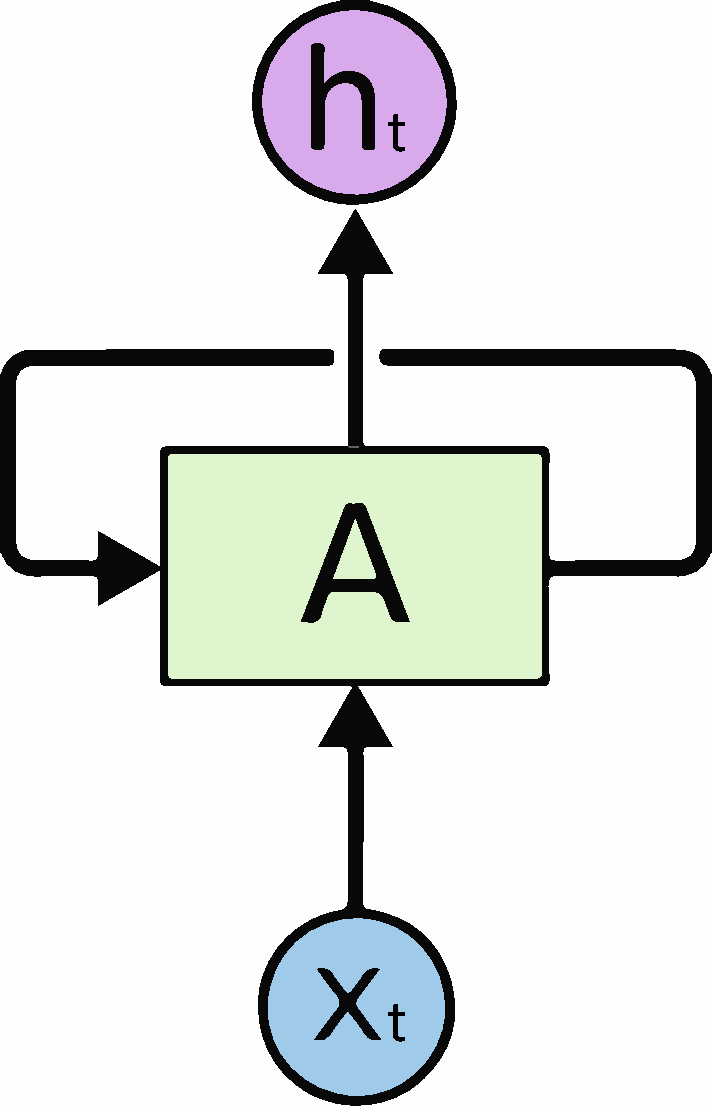
\includegraphics[width=0.3\linewidth]{img/RNN-rolled.png}}
    \end{center}
	\caption{Recurrent Neural Networks have loops. \todo{vlastni obrázek nebo citace \url{http://colah.github.io/posts/2015-08-Understanding-LSTMs/} }}
	\label{img:rnn-rolled}
\end{figure}

Funkce $f$ z rovnice \ref{figure:rnn} je nelineární funkcí a nejčastěji se používá jedna z funkcí \emph{sigmoid}, \emph{tanh} nebo \emph{relu} \ref{img:functions}. \todo{lepe popsat jednotlivé funkce a jejich výhody/nevýhody}

\begin{figure}[h]
    \begin{center}
            \tmpframe{\includegraphics[width=0.3\linewidth]{img/placeholder.pdf}}
            \tmpframe{\includegraphics[width=0.3\linewidth]{img/placeholder.pdf}}
            \tmpframe{\includegraphics[width=0.3\linewidth]{img/placeholder.pdf}}
    \end{center}
	\caption{\todo{vedle sebe obrazky funkci relu, tanh, sigmoid, idealne tri ruzny captions}}
	\label{img:functions}
\end{figure}


\begin{align}\label{figure:softmax}
  \sigma (\mathbf {z} )_{j}={\frac {e^{z_{j}}}{\sum _{k=1}^{K}e^{z_{k}}}}
\end{align}


\begin{figure}[h]
    \begin{center}
            \tmpframe{\includegraphics[width=1.0\linewidth]{img/RNN-unrolled.png}}
    \end{center}
	\caption{A recurrent neural network and the unfolding in time of the computation involved in its forward computation. \todo{vlastni obrázek nebo citace \url{http://colah.github.io/posts/2015-08-Understanding-LSTMs/} }}
	\label{img:rnn}
\end{figure}

\todo{doplnit rovnice a vysvětlení jak se to aplikuje dál, stejně tak obrázky s unrolled rnn a popisem toho jak zachovává nějakou informaci (třeba že podstatné jméno je mužské) skrze jednotlivé kroky (i když ne úplně přes vzdálené a tím se dostanu k long term dependencies)}


\todo{trénování rnn, back propagation through time, have difficulties (\url{http://proceedings.mlr.press/v28/pascanu13.pdf}) learning long term dependencies}
\todo{loss computing}
\todo{gradient computing}
\todo{související vanishing a exploding gradient problem popsáno v \cite{gradientProblems}, je to docela popsany i v nmtTutorial}
\todo{predchazeni vanish/exploding - lstm a gru, ktery s tim nejak pocitaji. Regularization - vysvětlit co to je}

\todo{zvlášť neuronky a to jakým způsobem se učí/optimlizují(gradient..) a pak až konkrétně rekurentní nebo rovnou rekurentní?}
\todo{deep, bi-directional}


\subsection{LSTM}\label{section:LSTM}
LSTM (Long short term memory \cite{LSTM} je varianta RNN řešící problém mizejícího gradientu a vzdálených závislostí \todo{lepší překlad pro long term dependencies?}.

\begin{align}
    f_{t}&=\sigma _{g}(W_{f}x_{t}+U_{f}h_{t-1}+b_{f})\\
    i_{t}&=\sigma _{g}(W_{i}x_{t}+U_{i}h_{t-1}+b_{i})\\
    o_{t}&=\sigma _{g}(W_{o}x_{t}+U_{o}h_{t-1}+b_{o})\\
    c_{t}&=f_{t}\circ c_{t-1}+i_{t}\circ \sigma_{c}(W_{c}x_{t}+U_{c}h_{t-1}+b_{c})\\
    h_{t}&=o_{t}\circ \sigma _{h}(c_{t})
\end{align}

\subsection{GRU}\label{section:GRU}


\subsection{Trénování}
\subsection{Global optimization methods viz wiki on RNN}

\section{Word embeddings}
\todo{souvislost s jazykovymy modely}
\blind{2}
\begin{figure}
    \begin{center}
            \tmpframe{\includegraphics[width=0.5\linewidth]{img/placeholder.pdf}}
    \end{center}
	\caption{One image. \todo{Napsat pořádný titulek}}
	\label{img:TODO}
\end{figure}
\todo{subsection nebo itemize?}
\subsection{word2vec}
\blind{1}
\subsection{glove}
\blind{1}
\subsection{fasttext}
\blind{1}

\section{Modely seq2seq}
\blind{2}
\begin{figure}
    \begin{center}
            \tmpframe{\includegraphics[width=0.5\linewidth]{img/placeholder.pdf}}
    \end{center}
	\caption{One image. \todo{Napsat pořádný titulek}}
	\label{img:TODO}
\end{figure}
\subsection{Encoder-decoder architektura}
\begin{figure}
    \begin{center}
            \tmpframe{\includegraphics[width=0.5\linewidth]{img/placeholder.pdf}}
    \end{center}
	\caption{One image. \todo{Napsat pořádný titulek}}
	\label{img:TODO}
\end{figure}
\blind{3}
\subsection{Attention/Pozornost}




\section{Frameworky}
Chci popsat různé frameworky ze kterých jsem vybíral a vysvětlit proč jsem zvolil Keras.
\blind{2}
\todo{subsection nebo itemize?, mozna nejake obrazky}
\subsection{Tensorflow}
\blind{1}
\subsection{Theano}
\blind{1}
\subsection{CNTK}
\blind{1}
\subsection{Keras}
\blind{1}

\chapter{Návrh systému (Praxe, nové myšlenky, které práce přináší)}
Rozhodl jsem se.
Vymyslel jsem.
Rozvrhl jsem.
Vypočítal jsem.
Odvodil jsem.
Zjednodušil jsem.
Vylepšil jsem.
Navrhl jsem.
Zjistil jsem.
Vyzkoumal jsem.

\section{Neformální návrh systému}
Vyberu a použiju nějký dataset, který obsahuje zarovnané věty se stejným významem ve dvou různých jazycích. Tyto věty za pomocí nějakého tokenizeru rozdělím na jednotlivé tokeny (slova/značky jako vykřičník) a to bude vstup pro překládací model.

Model bude sestavený z Embedding části, která převádí slova do vektorů s nějakým významem -- tedy z toho může neuronová síť něco použít, narozdíl od toho kdyby slova reprezentoval jen index. Pro tento účel použiju přednaučené embeddings od Facebooku (fasttext). Dále v modelu Encoder, který se sestává z vrstvy/vrstev rekurentní neuronové sítě (LSTM). Tímto Encoderem projde celá sekvence embeddings a vznikne tak "thought vector", což je význam dané věty převedený do nějakého velkého vektoru (latent dimension?). Z tohoto vektoru/prostoru pak Dekodér, což je také vrstva/vrstvy LSTM postupně generuje překlad po jednotlivých slovech. Na vstup nejdříve dostane startovací značku a jeho vnitřní stav (memory cell) se inicializuje stavem encoderu. Po každém vygenerovaném slovu dostane toto slovo na vstup a takto generuje tak dlouho, dokud nevygeneruje značku konec sekvence. Výstup z dekoderu je vrstva softmax o velikosti slovníku jazyka do kterého se překládá. Generovaná slova se vyberou buď jednoduchým argmaxem, tedy vybere se vždycky slovo s největší vycházející pravděpodobností a nebo nějakou pokročilejší metodou, jako je beam search.


\section{Baseline systém v Moses}
\todo{Jak rozlišit návrh a realizaci?}
\blind{3}

\section{Dataset/y}
Jejich struktura, jak je zpracuji a použiji
\blind{2}
\begin{figure}
    \begin{center}
            \tmpframe{\includegraphics[width=0.5\linewidth]{img/placeholder.pdf}}
    \end{center}
	\caption{One image. \todo{ukázka ze souborů různých jazyků z jednoho datasetu}}
	\label{img:TODO}
\end{figure}


\chapter{Implementace, experimenty, vyhodnocení}
Naprogramoval jsem.
Posbíral jsem data.
Pustil jsem to.
Výsledky jsou takové.
Je to tak a tak rychlé.

\subsection{Bucketing}
A padding. Rozdělení sekvencí na skupiny podle délky, abych nepaddingoval zbytečně a tím neplýtval výkon.

\section{skóre BLEU}
\blind{1}
\todo{vysazet hezky vzorce}

\chapter{Závěr}
\begin{itemize}
  \item Autor se ohlíží za tím, co udělal: „V práci je. Hlavní úspěchy jsou. Důležitými výsledky jsou. Podařilo se.“
  \item Autor uvede nápady, které nestihl realizovat v podobě možností pokračování: „Ještě by šlo zkusit. Kdybych byl na začátku věděl, co vím teď, dělal bych.“
  \item Autor (ve vlastním zájmu) rekapituluje, jak bylo naplněno zadání práce.
\end{itemize}

\subsection{Plány do budoucna}
\begin{itemize}
    \item použití bidirectional první vrstvy encoderu, pro lepší zachování contextu \cite{googleBridgingGap} na místo použití obrácených vstupů
    \item použití wordpieces \cite{googleBridgingGap} místo celých slov pro lepší handling rare words
    \item přidat attention \cite{attention}
    \item přidat beam search \cite{nmtTutorial}, sehnat původní článek co přinesl beam search
\end{itemize}
